\section{Setup} \label{sec:setup}
\subsection{Definitions}
Throughout the paper we look at curved folded surfaces as piecewise $C^2$ developable surfaces, whose discontinuities are focused along creases. We assume that these creases are $C^2$ curves that may intersect one another, and we call these intersections \textit{crease vertices}. These curves segment the surface into various disconnected components, which we call curved patches. We also assume that these curved patches are $C^2$, i.e. though the folding operation creates discontinuities along the patches, viewed separately they are deformed by $C^2$ deformations. Throughout the paper we will often visualize the crease pattern itself by looking at the isometric flat surface together with its curved creases (see \figref{fig:crease_pattern}).
\begin{figure} [h]
	\centering
	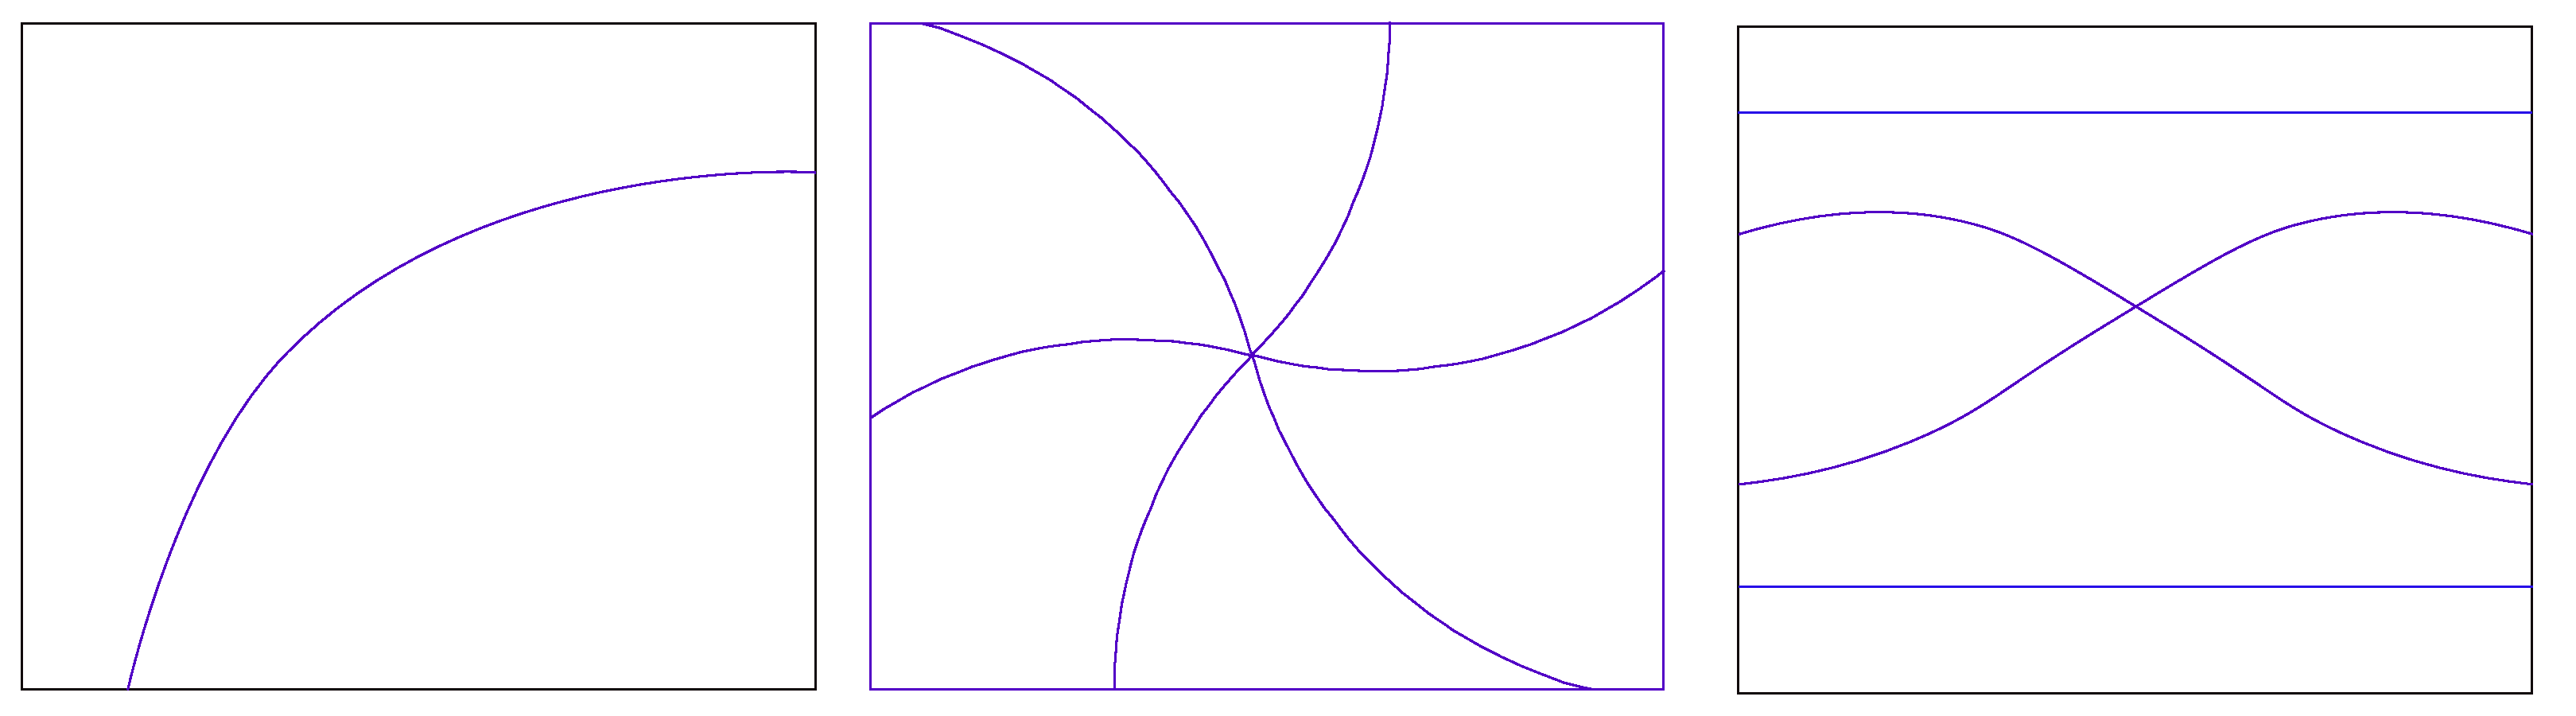
\includegraphics[width=\linewidth]{figures/crease_patterns}
	\caption{Curved and straight crease patterns, decomposing a pattern into multiple components and intersecting at crease vertices.}
	\label{fig:crease_pattern}
\end{figure}

\subsection{Model} \label{sec:model}
We follow the work of \cite{rabi2018shape} by modeling each smooth patch as a discrete orthogonal geodesic net (see \figref{fig:curve_on_dog}). We represent a crease as piecewise linear curves, whose points $c(i)$ are represented by the curves' intersection point with the grid edges. Each point $c(i)$ is a linear combination of two vertices on a DOG: $c(i) = t v_i + (1-t)v_j,$ where $0 \leq t \leq 1$ and $v_i,v_j$ are too neighbour vertices on the grid.  Each point on a crease lies on each of the $m \geq 2$ different patches, essentially duplicated. If $c(i)^1,c(i)^2,....,c(i)^m$ are the representation of $c(i)$ on the different patches, we enforce constrain these duplicated points have equal coordinates (see \figref{fig:curve_on_dog}).
We trivially extend the represntation at \cite{rabi2018shape} to support intersecting curves by adding grid lines at crease vertices (see \figref{fig:piecewise_dog_from_crease} and \figref{fig:curve_on_dog}).

\begin{figure} [h]
	\centering
	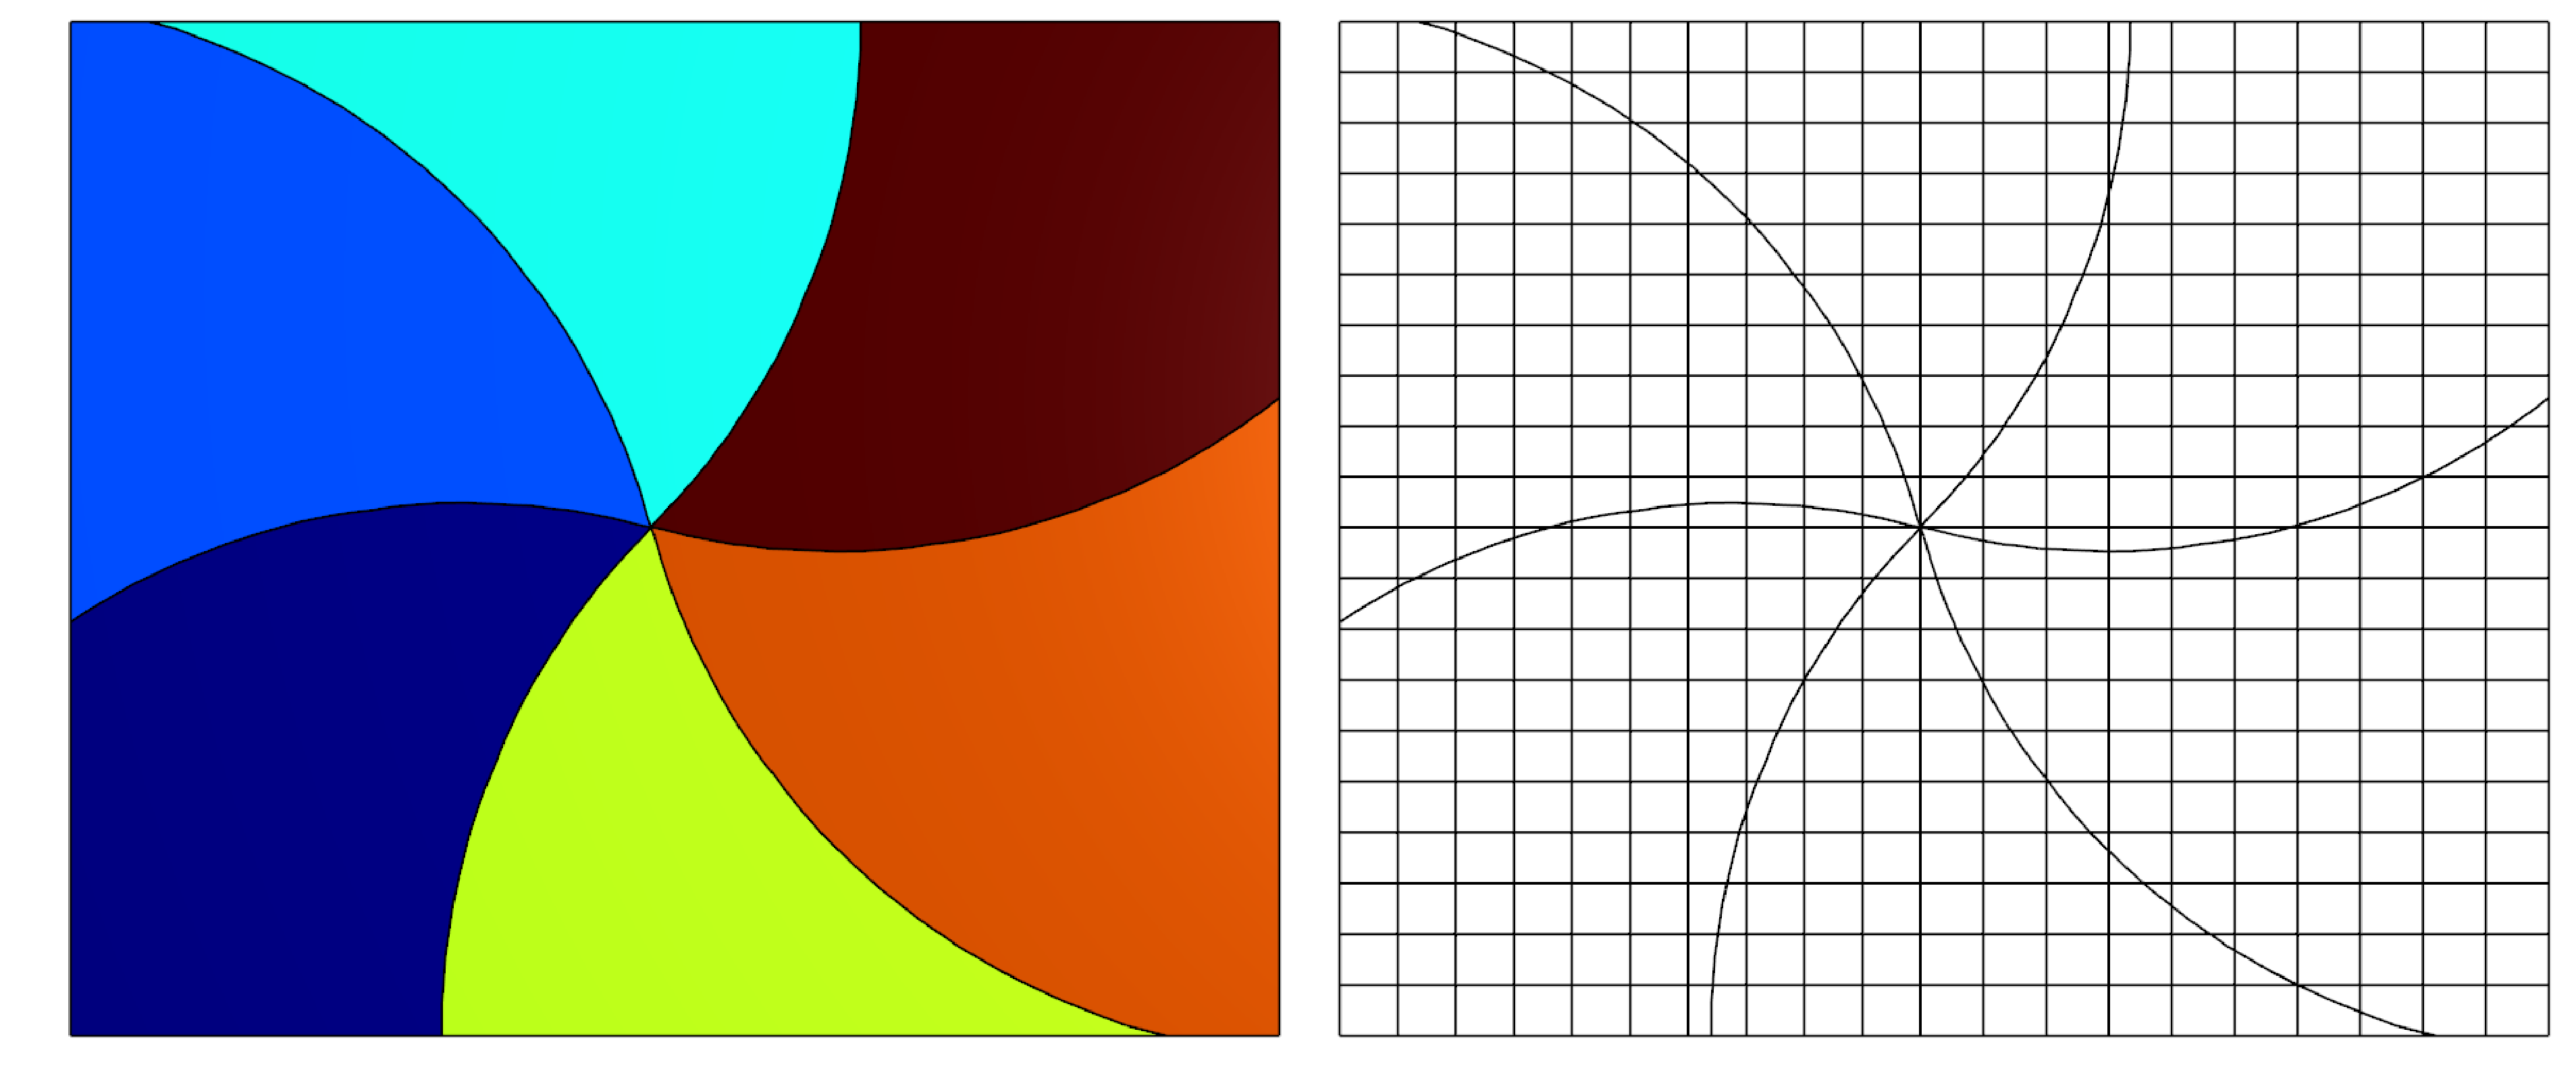
\includegraphics[width=0.8\linewidth]{figures/piecewise_dog_from_crease}
	\caption{Given a crease pattern, we create a DOG for each segment (colored differently), and use the boundary constraints as done in \cite{rabi2018shape}.}
	\label{fig:piecewise_dog_from_crease}
\end{figure}

\begin{figure} [h]
	\centering
	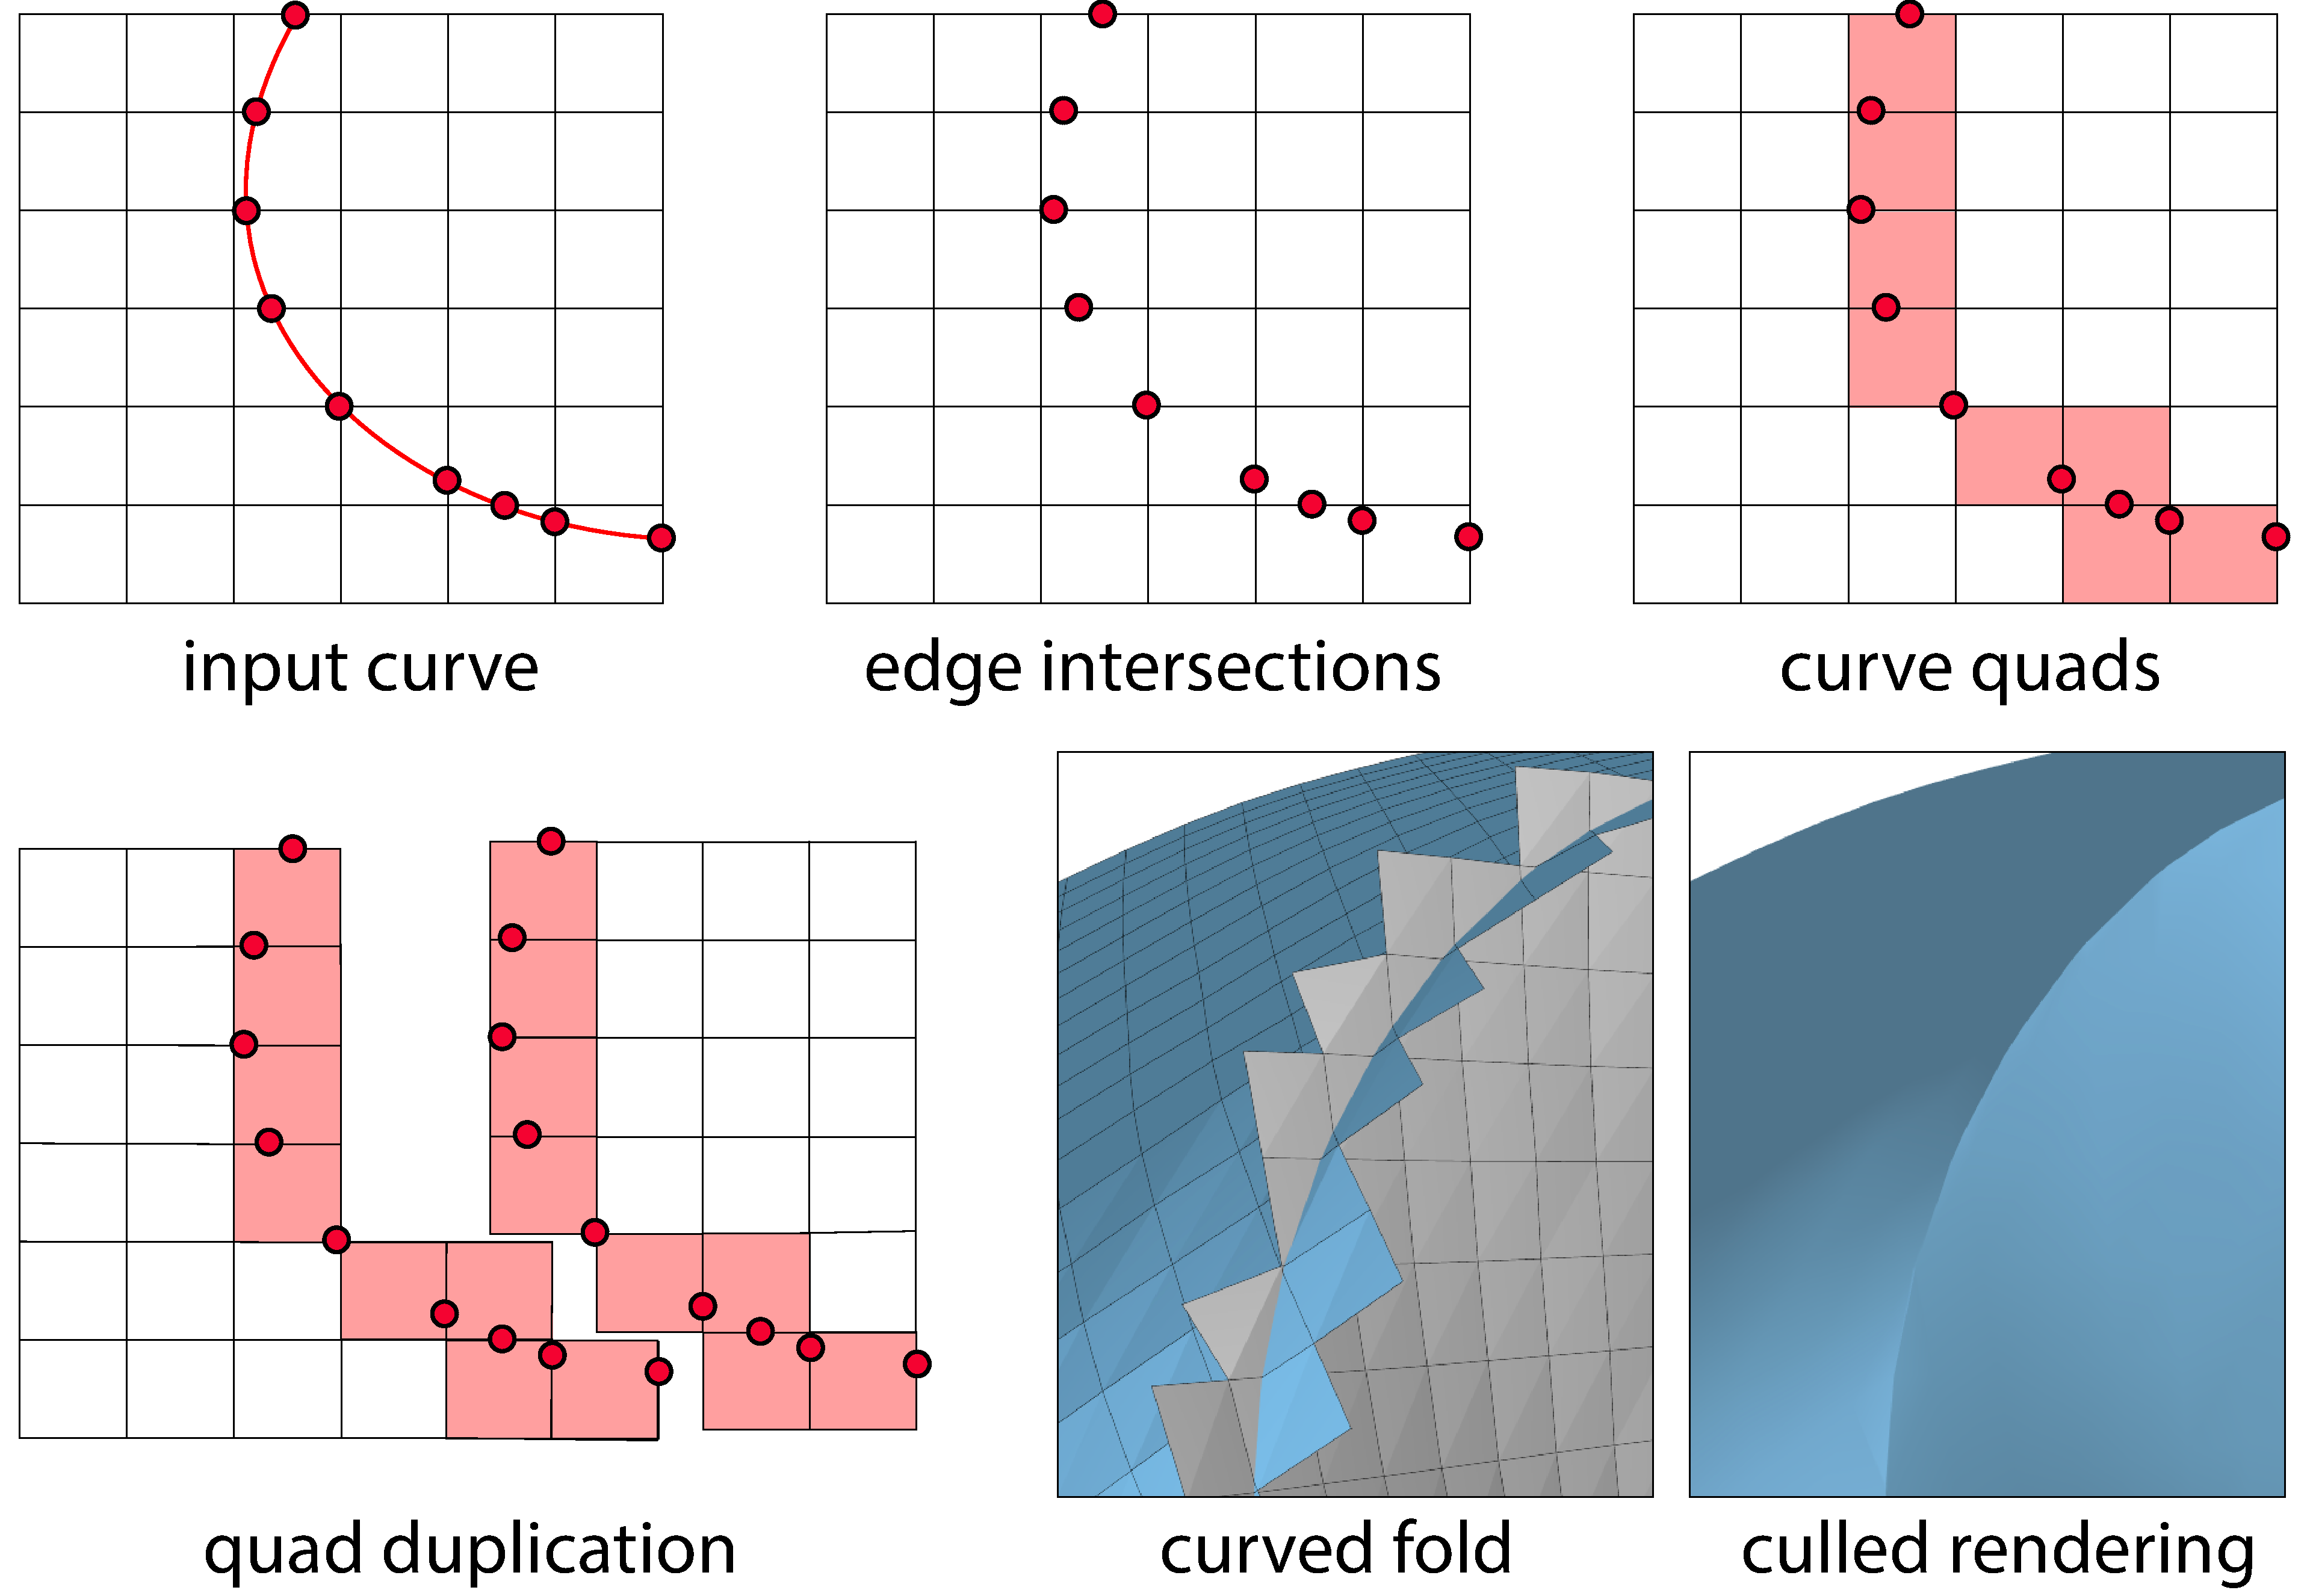
\includegraphics[width=0.8\linewidth]{figures/curve_on_dog}
	\caption{Picture taken from \cite{rabi2018shape}.}
	\label{fig:curve_on_dog}
\end{figure}

\subsection{Desiderata}
Our goal is to develop tools for the exploration of curved folded shapes on top of piecewise DOGs by means of deformations. Our choices are guided by the following ground rules for deforming DOGs:
\begin{enumerate}
  \item Perform homotopy based optimization \label{homotopy_opt}
  \item Minimally constrain DOGs \label{minimal_const}
%  \item Use accurate functionals \label{accurate_func}
%  \item Use simple functionals
\end{enumerate}
\textbf{Homotopy based optimization} is motivated both theoretically and empirically; Modeling DOGs requires solving highly constrained and non linear optimization problems, yet the theory of DOGs guarantees the existence of nearby solutions if one starts at a feasible point. In fact, generally the shape space of DOGs is a smooth manifold \cite{rabi2018shape}. This observation is worthwhile in practice; DOGs exploration was demonstrated to perform well using smooth flow, or homotopy based optimization methods both for handle based editing tasks as well for more complicated deformations such as curve-constraining flows \cite{rabi2018shape}. \\
\textbf{Minimally constrain DOGs.} As DOGs are already heavily constrained, one needs to carefully choose which quantities to constrain by hard constraints, and which ones should be optimized using soft constraints. This is essential to avoid locking, or ill-posed problems in case the constraint gradients are linearly independent \cite{rabi2018shape}. In particular, the rigidity analysis in \cite{rabi18} demonstrates that one cannot fix all edge length exactly, or likewise demand a DOG to also be a Chebyshev net. We note however that this can be done approximately and to a low tolerance as a DOG is a chebyshev at the smooth limit and at the smooth limit there is a rich set of exact isometries. The folding constraints at \secref{sec:folding} where chosen such that they could be satisfied \textit{exactly}, and so that in practice they vanish once the surface is sufficiently folded, just like a piecewise smooth curved folded surface. \\
%\textbf{Accurate functionals.} We look for constraints and objectives that are accurate and as often in the case with DOG objectives, converge under sampling of a smooth orthogonal geodesic net \cite{rabi18,rabi2018shape}. \\
%\textbf{Simple functionals.} We strongly prefer sparser objectives with a lower degree as possible. To that end, we leverage the regularity of the DOG meshing and theory on smooth orthogonal geodesic nets in our derivations. \\